\message{ !name(iceWater.tex)}
\message{ !name(iceWater.tex) !offset(-2) }
\chapter{SIMULATIONS OF SOLID-LIQUID FRICTION AT ICE-I$_\mathrm{h}$ /WATER INTERFACES}

 We have investigated the structural and dynamic properties of the
  basal and prismatic facets of the ice I$_\mathrm{h}$ / water
  interface when the solid phase is drawn through the liquid
  (i.e. sheared relative to the fluid phase). To impose the shear, we
  utilized a velocity-shearing and scaling (VSS) approach to reverse
  non-equilibrium molecular dynamics (RNEMD).  This method can create
  simultaneous temperature and velocity gradients and allow the
  measurement of transport properties at interfaces.  The interfacial
  width was found to be independent of the relative velocity of the
  ice and liquid layers over a wide range of shear rates.  Decays of
  molecular orientational time correlation functions gave similar
  estimates for the width of the interfaces, although the short- and
  longer-time decay components behave differently closer to the
  interface.  Although both facets of ice are in ``stick'' boundary
  conditions in liquid water, the solid-liquid friction coefficients
  were found to be significantly different for the basal and prismatic
  facets of ice.


\section{Introduction}
%-----Outline of Intro---------------
% in general, ice/water interface is important b/c ....
% here are some people who have worked on ice/water, trying to understand the processes above ....
% with the recent development of VSS-RNEMD, we can now look at the shearing problem
% talk about what we will present in this paper
% -------End Intro------------------

%Gay02: cites many other ice/water papers, make sure to cite them.

Understanding the ice/water interface is essential for explaining
complex processes such as nucleation and crystal
growth,\cite{Han92,Granasy95,Vanfleet95} crystal
melting,\cite{Weber83,Han92,Sakai96,Sakai96B} and some fascinating
biological processes, such as the behavior of the antifreeze proteins
found in winter flounder,\cite{Wierzbicki07, Chapsky97} and certain
terrestrial arthropods.\cite{Duman:2001qy,Meister29012013} There has
been significant progress on understanding the structure and dynamics
of quiescent ice/water interfaces utilizing both theory and
experiment.  Haymet \emph{et al.} have done extensive work on ice I$_\mathrm{h}$,
including characterizing and determining the width of the ice/water
interface for the SPC,\cite{Karim90} SPC/E,\cite{Gay02,Bryk02} CF1,\cite{Hayward01,Hayward02} and TIP4P~\cite{Karim88} models for
water.
More recently, Haymet \emph{et al.} have investigated the effects
cations and anions have on crystal
nucleation.\cite{Bryk04,Smith05,Wilson08,Wilson10} Nada \emph{et al.}
have also studied ice/water
interfaces,\cite{Nada95,Nada00,Nada03,Nada12} and have found that the
differential growth rates of the facets of ice I$_\mathrm{h}$ are due to the the
reordering of the hydrogen bonding network.\cite{Nada05}

The movement of liquid water over the facets of ice has been less
thoroughly studied than the quiescent surfaces. This process is
potentially important in understanding transport of large blocks of
ice in water (which has important implications in the earth sciences),
as well as the relative motion of crystal-crystal interfaces that have
been separated by nanometer-scale fluid domains.  In addition to
understanding both the structure and thickness of the interfacial
regions, it is important to understand the molecular origin of
friction, drag, and other changes in dynamical properties of the
liquid in the regions close to the surface that are altered by the
presence of a shearing of the bulk fluid relative to the solid phase.

In this work, we apply a recently-developed velocity shearing and
scaling approach to reverse non-equilibrium molecular dynamics
(VSS-RNEMD). This method makes it possible to calculate transport
properties like the interfacial thermal conductance across
heterogeneous interfaces,\cite{Kuang12} and can create simultaneous
temperature and velocity gradients and allow the measurement of
friction and thermal transport properties at interfaces.  This has
allowed us to investigate the width of the ice/water interface as the
ice is sheared through the liquid, while simultaneously imposing a
weak thermal gradient to prevent frictional heating of the interface.
In the sections that follow, we discuss the methodology for creating
and simulating ice/water interfaces under shear and provide results
from both structural and dynamical correlation functions.  We also
show that the solid-liquid interfacial friction coefficient depends
sensitively on the details of the surface morphology.

\section{Methodology}

\subsection{Stable ice I$_\mathrm{h}$ / water interfaces under shear}

The structure of ice I$_\mathrm{h}$ is well understood; it
crystallizes in a hexagonal space group P$6_3/mmc$, and the hexagonal
crystals of ice have two faces that are commonly exposed, the basal
face $\{0~0~0~1\}$, which forms the top and bottom of each hexagonal
plate, and the prismatic $\{1~0~\bar{1}~0\}$ face which forms the
sides of the plate. Other less-common, but still important, faces of
ice I$_\mathrm{h}$ are the secondary prism, $\{1~1~\bar{2}~0\}$, and
pyramidal, $\{2~0~\bar{2}~1\}$, faces.  Ice I$_\mathrm{h}$ is normally
proton disordered in bulk crystals, although the surfaces probably
have a preference for proton ordering along strips of dangling H-atoms
and Oxygen lone pairs.\cite{Buch:2008fk}

\begin{table}[h]
\centering
  \caption{Mapping between the Miller indices of four facets of ice in
    the $P6_3/mmc$ crystal system to the orthorhombic $P2_12_12_1$
    system in reference \bibpunct{}{}{,}{n}{}{,} \protect\citep{Hirsch04}.}
\label{tab:equiv}
\begin{tabular}{|ccc|} \hline
 & hexagonal & orthorhombic \\
 & ($P6_3/mmc$) & ($P2_12_12_1$) \\
 crystal face  & Miller indices & equivalent \\ \hline
basal & $\{0~0~0~1\}$ & $\{0~0~1\}$ \\
prism & $\{1~0~\bar{1}~0\}$ & $\{1~0~0\}$ \\
secondary prism & $\{1~1~\bar{2}~0\}$ & $\{1~3~0\}$ \\
pyramidal & $\{2~0~\bar{2}~1\}$ & $\{2~0~1\}$ \\ \hline
\end{tabular}
\end{table}
For small simulated ice interfaces, it is useful to work with
proton-ordered, but zero-dipole crystal that exposes these strips of
dangling H-atoms and lone pairs.  When placing another material in
contact with one of the ice crystalline planes, it is also quite
useful to have an orthorhombic (rectangular) box. Recent work by
Hirsch and Ojam\"{a}e describes a number of alternative crystal
systems for proton-ordered bulk ice I$_\mathrm{h}$ using orthorhombic
cells.\cite{Hirsch04}

In this work, we are using Hirsch and Ojam\"{a}e's structure 6 which
is an orthorhombic cell ($P2_12_12_1$) that produces a proton-ordered
version of ice I$_\mathrm{h}$.  Table \ref{tab:equiv} contains a
mapping between the Miller indices of common ice facets in the
P$6_3/mmc$ crystal system and those in the Hirsch and Ojam\"{a}e
$P2_12_12_1$ system.

Structure 6 from the Hirsch and Ojam\"{a}e paper has lattice
parameters $a = 4.49225$ \AA\ , $b = 7.78080$ \AA\ , $c = 7.33581$ \AA\
and two water molecules whose atoms reside at fractional coordinates
given in table \ref{tab:p212121}. To construct the basal and prismatic
interfaces, these crystallographic coordinates were used to construct
an orthorhombic unit cell which was then replicated in all three
dimensions yielding a proton-ordered block of ice I$_{h}$. To expose
the desired face, the orthorhombic representation was then cut along
the ($001$) or ($100$) planes for the basal and prismatic faces
respectively. The resulting block was rotated so that the exposed
faces were aligned with the $z$-axis normal to the exposed face. The
block was then cut along two perpendicular directions in a way that
allowed for perfect periodic replication in the $x$ and $y$ axes,
creating a slab with either the basal or prismatic faces exposed along
the $z$ axis. The slab was then replicated in the $x$ and $y$
dimensions until a desired sample size was obtained.

\begin{table}[h]
\centering
  \caption{Fractional coordinates for water in the orthorhombic
    $P2_12_12_1$ system for ice I$_\mathrm{h}$ in reference \bibpunct{}{}{,}{n}{}{,} \protect\citep{Hirsch04}.}
\label{tab:p212121}
\begin{tabular}{|cccc|}  \hline
atom type & x & y & z \\ \hline
 O & 0.7500 & 0.1667 & 0.4375 \\
 H & 0.5735 & 0.2202 & 0.4836 \\
 H & 0.7420 & 0.0517 & 0.4836 \\
 O & 0.2500 & 0.6667 & 0.4375 \\
 H & 0.2580 & 0.6693 & 0.3071 \\
 H & 0.4265 & 0.7255 & 0.4756 \\ \hline
\end{tabular}
\end{table}

Our ice / water interfaces were created using a box of liquid water
that had the same dimensions (in $x$ and $y$) as the ice block.
Although the experimental solid/liquid coexistence temperature under
atmospheric pressure is close to 273~K, Haymet \emph{et al.} have done
extensive work on characterizing the ice/water interface, and find
that the coexistence temperature for simulated water is often quite a
bit different.\cite{Karim88,Karim90,Hayward01,Bryk02,Hayward02} They
have found that for the SPC/E water model,\cite{Berendsen87} which is
also used in this study, the ice/water interface is most stable at
225~$\pm$5~K.\cite{Bryk02} This liquid box was therefore equilibrated at
225~K and 1~atm of pressure in the NPAT ensemble (with the $z$ axis
allowed to fluctuate to equilibrate to the correct pressure).  The
liquid and solid systems were combined by carving out any water
molecule from the liquid simulation cell that was within 3~\AA\ of any
atom in the ice slab. The resulting basal system was $23.87 \times 35.83
\times 98.64$ \AA\ with 900 SPC/E molecules in the ice slab, and 1846 in
the liquid phase.  Similarly, the prismatic system was $36.12 \times 36.43
\times 86.10$ \AA\ with 1000 SPC/E molecules in the ice slab and 2684 in
the liquid.

Molecular translation and orientational restraints were applied in the
early stages of equilibration to prevent melting of the ice slab.
These restraints were removed during NVT equilibration, well before
data collection was carried out.  

\subsection{Shearing ice / water interfaces without bulk melting}

As a solid is dragged through a liquid, there is frictional heating
that will act to melt the interface.  To study the behavior of the
interface under a shear stress without causing the interface to melt,
it is necessary to apply a weak thermal gradient in combination with
the momentum gradient.  This can be accomplished using the velocity
shearing and scaling (VSS) variant of reverse non-equilibrium
molecular dynamics (RNEMD), which utilizes a series of simultaneous
velocity exchanges between two regions within the simulation
cell.\cite{Kuang12} One of these regions is centered within the ice
slab, while the other is centrally located in the liquid
region. VSS-RNEMD provides a set of conservation constraints for
creating either a momentum flux or a thermal flux (or both
simultaneously) between the two slabs.  Satisfying the constraint
equations ensures that the new configurations are sampled from the
same NVE ensemble as before the VSS move.

The VSS moves are applied periodically to scale and shift the particle
velocities ($\mathbf{v}_i$ and $\mathbf{v}_j$) in two slabs ($H$ and
$C$) which are separated by half of the simulation box,
\begin{displaymath}
\begin{array}{rclcl}

 & \underline{\mathrm{shearing}} & &
 \underline{~~~~~~~~~~~~\mathrm{scaling}~~~~~~~~~~~~} \\
\mathbf{v}_i \leftarrow & 
  \mathbf{a}_c\ & + & c\cdot\left(\mathbf{v}_i - \langle\mathbf{v}_c
  \rangle\right)  +  \langle\mathbf{v}_c\rangle \\
\mathbf{v}_j \leftarrow & 
  \mathbf{a}_h & + & h\cdot\left(\mathbf{v}_j - \langle\mathbf{v}_h
    \rangle\right) + \langle\mathbf{v}_h\rangle .

\end{array}
\end{displaymath}
Here $\langle\mathbf{v}_c\rangle$ and $\langle\mathbf{v}_h\rangle$ are
the center of mass velocities in the $C$ and $H$ slabs, respectively.
Within the two slabs, particles receive incremental changes or a
``shear'' to their velocities.  The amount of shear is governed by the
imposed momentum flux, $\mathbf{j}_z(\mathbf{p})$
\begin{eqnarray}
\mathbf{a}_c & = & - \mathbf{j}_z(\mathbf{p}) \Delta t / M_c \label{vss1}\\
\mathbf{a}_h & = & + \mathbf{j}_z(\mathbf{p}) \Delta t / M_h \label{vss2}
\end{eqnarray}
where $M_{\{c,h\}}$ is the total mass of particles within each of the
slabs and $\Delta t$ is the interval between two separate operations.

To simultaneously impose a thermal flux ($J_z$) between the slabs we
use energy conservation constraints,
\begin{eqnarray}
K_c - J_z\Delta t & = & c^2 (K_c - \frac{1}{2}M_c \langle\mathbf{v}_c
\rangle^2) + \frac{1}{2}M_c (\langle \mathbf{v}_c \rangle + \mathbf{a}_c)^2 \label{vss3}\\
K_h + J_z\Delta t & = & h^2 (K_h - \frac{1}{2}M_h \langle\mathbf{v}_h
\rangle^2) + \frac{1}{2}M_h (\langle \mathbf{v}_h \rangle +
\mathbf{a}_h)^2 \label{vss4}.
\label{constraint}
\end{eqnarray}
Simultaneous solution of these quadratic formulae for the scaling
coefficients, $c$ and $h$, will ensure that the simulation samples from
the original microcanonical (NVE) ensemble.  Here $K_{\{c,h\}}$ is the
instantaneous translational kinetic energy of each slab.  At each time
interval, it is a simple matter to solve for $c$, $h$, $\mathbf{a}_c$,
and $\mathbf{a}_h$, subject to the imposed momentum flux,
$j_z(\mathbf{p})$, and thermal flux, $J_z$, values.  Since the VSS
operations do not change the kinetic energy due to orientational
degrees of freedom or the potential energy of a system, configurations
after the VSS move have exactly the same energy (and linear
momentum) as before the move.

As the simulation progresses, the VSS moves are performed on a regular
basis, and the system develops a thermal and/or velocity gradient in
response to the applied flux.  In a bulk material, it is quite simple
to use the slope of the temperature or velocity gradients to obtain
either the thermal conductivity or shear viscosity.

The VSS-RNEMD approach is versatile in that it may be used to
implement thermal and shear transport simultaneously.  Perturbations
of velocities away from the ideal Maxwell-Boltzmann distributions are
minimal, as is thermal anisotropy.  This ability to generate
simultaneous thermal and shear fluxes has been previously utilized to
map out the shear viscosity of SPC/E water over a wide range of
temperatures (90~K) with a single 1~ns simulation.\cite{Kuang12}

For this work, we are using the VSS-RNEMD method primarily to generate
a shear between the ice slab and the liquid phase, while using a weak
thermal gradient to maintain the interface at the 225~K target
value. This ensures minimal melting of the bulk ice phase and allows
us to control the exact temperature of the interface.

\subsection{Computational Details}
All simulations were performed using OpenMD,\cite{OOPSE,openmd} with a
time step of 2 fs and periodic boundary conditions in all three
dimensions.  Electrostatics were handled using the damped-shifted
force real-space electrostatic kernel.\cite{Ewald} The systems were
divided into 100 bins along the $z$-axis for the VSS-RNEMD moves,
which were attempted every 50~fs. 

The interfaces were equilibrated for a total of 10 ns at equilibrium
conditions before being exposed to either a shear or thermal gradient.
This consisted of 5 ns under a constant temperature (NVT) integrator
set to 225K followed by 5 ns under a microcanonical integrator.  Weak
thermal gradients were allowed to develop using the VSS-RNEMD (NVE)
integrator using a small thermal flux ($-2.0\times 10^{-6}$
kcal/mol/\AA$^2$/fs) for a duration of 5 ns to allow the gradient to
stabilize.  The resulting temperature gradient was $\approx$ 10K over
the entire 100 \AA\  box length, which was sufficient to keep the
temperature at the interface within $\pm 1$ K of the 225K target.

Velocity gradients were then imposed using the VSS-RNEMD (NVE)
integrator with a range of momentum fluxes.  These gradients were
allowed to stabilize for 1~ns before data collection began. Once
established, four successive 0.5~ns runs were performed for each shear
rate.  During these simulations, snapshots of the system were taken
every 1~ps, and statistics on the structure and dynamics in each bin
were accumulated throughout the simulations.  Although there was some
small variation in the measured interfacial width between succcessive
runs, no indication of bulk melting (or crystallization) was observed.

\section{Results and discussion}

\subsection{Interfacial width}
Any order parameter or time correlation function that changes as one
crosses an interface from a bulk liquid to a solid can be used to
measure the width of the interface.  In previous work on the ice/water
interface, Haymet {\it et al.}\cite{Bryk02} have utilized structural
features (including the density) as well as dynamic properties
(including the diffusion constant) to estimate the width of the
interfaces for a number of facets of the ice crystals.  Because
VSS-RNEMD imposes a lateral flow, parameters that depend on
translational motion of the molecules (e.g. diffusion) may be
artificially skewed by the RNEMD moves.  A structural parameter is not
influenced by the RNEMD perturbations to the same degree. Here, we
have used the local tetrahedral order parameter as described by
Kumar\cite{Kumar09} and Errington\cite{Errington01} as our principal
measure of the interfacial width.  A previous study by Bryk and Haymet
also used local tetrahedrality as an order parameter for ice/water
interfaces.\cite{Bryk2004b}

The local tetrahedral order parameter, $q(z)$, is given by
\begin{equation}
q(z) = \int_0^L \sum_{k=1}^{N} \Bigg(1 -\frac{3}{8}\sum_{i=1}^{3}
\sum_{j=i+1}^{4} \bigg(\cos\psi_{ikj}+\frac{1}{3}\bigg)^2\Bigg)
\delta(z_{k}-z)\mathrm{d}z \Bigg/ N_z
\label{eq:qz}
\end{equation}
where $\psi_{ikj}$ is the angle formed between the oxygen site on
central molecule $k$, and the oxygen sites on two of the four closest
molecules, $i$ and $j$.  Molecules $i$ and $j$ are further restricted
to lie withing the first peak in the pair distribution function for
molecule $k$ (typically $<$ 3.41 \AA\ for water).  $N_z = \int
\delta(z_k - z) \mathrm{d}z$ is a normalization factor to account for
the varying population of molecules within each finite-width bin.  The
local tetrahedral order parameter has a range of $(0,1)$, where the
larger values of $q$ indicate a larger degree of tetrahedral ordering
of the local environment.  In perfect ice I$_\mathrm{h}$ structures,
the parameter can approach 1 at low temperatures, while in liquid
water, the ordering is significantly less tetrahedral, and values of
$q(z) \approx 0.75$ are more common.

To estimate the interfacial width, the system was divided into 100
bins along the $z$-dimension.  The $q_{z}$ function was time-averaged
to give yield a tetrahedrality profile of the system. The profile was
then fit to a hyperbolic tangent that smoothly links the liquid and
solid states,
\begin{equation}\label{tet_fit}
q(z) \approx
q_{liq}+\frac{q_{ice}-q_{liq}}{2}\left[\tanh\left(\frac{z-l}{w}\right)-\tanh\left(\frac{z-r}{w}\right)\right]+\beta\left|z-
\frac{r+l}{2}\right|.
\end{equation}
Here $q_{liq}$ and $q_{ice}$ are the local tetrahedral order parameter
for the bulk liquid and ice domains, respectively, $w$ is the width of
the interface.  $l$ and $r$ are the midpoints of the left and right
interfaces, respectively.  The last term in eq. \eqref{tet_fit}
accounts for the influence that the weak thermal gradient has on the
tetrahedrality profile in the liquid region. 

In Figures \ref{fig:bComic} and \ref{fig:pComic} we see the
$z$-coordinate profiles for tetrahedrality, temperature, and the
$x$-component of the velocity for the basal and prismatic interfaces.
The lower panels show the $q(z)$ (black circles) along with the
hyperbolic tangent fits (red lines). In the liquid region, the local
tetrahedral order parameter, $q(z) \approx 0.75$ while in the
crystalline region, $q(z) \approx 0.94$, indicating a more tetrahedral
environment.  The vertical dotted lines denote the midpoint of the
interfaces ($r$ and $l$ in eq. \eqref{tet_fit}). The weak thermal
gradient applied to the systems in order to keep the interface at
225~$\pm$~5K, can be seen in middle panels.  The transverse velocity
profile is shown in the upper panels.  It is clear from the upper
panels that water molecules in close proximity to the surface (i.e.
within 10~\AA\ to 15~\AA~of the interfaces) have transverse velocities
quite close to the velocities within the ice block.  There is no
velocity discontinuity at the interface, which indicates that the
shearing of ice/water interfaces occurs in the ``stick'' or no-slip
boundary conditions.

\begin{figure}
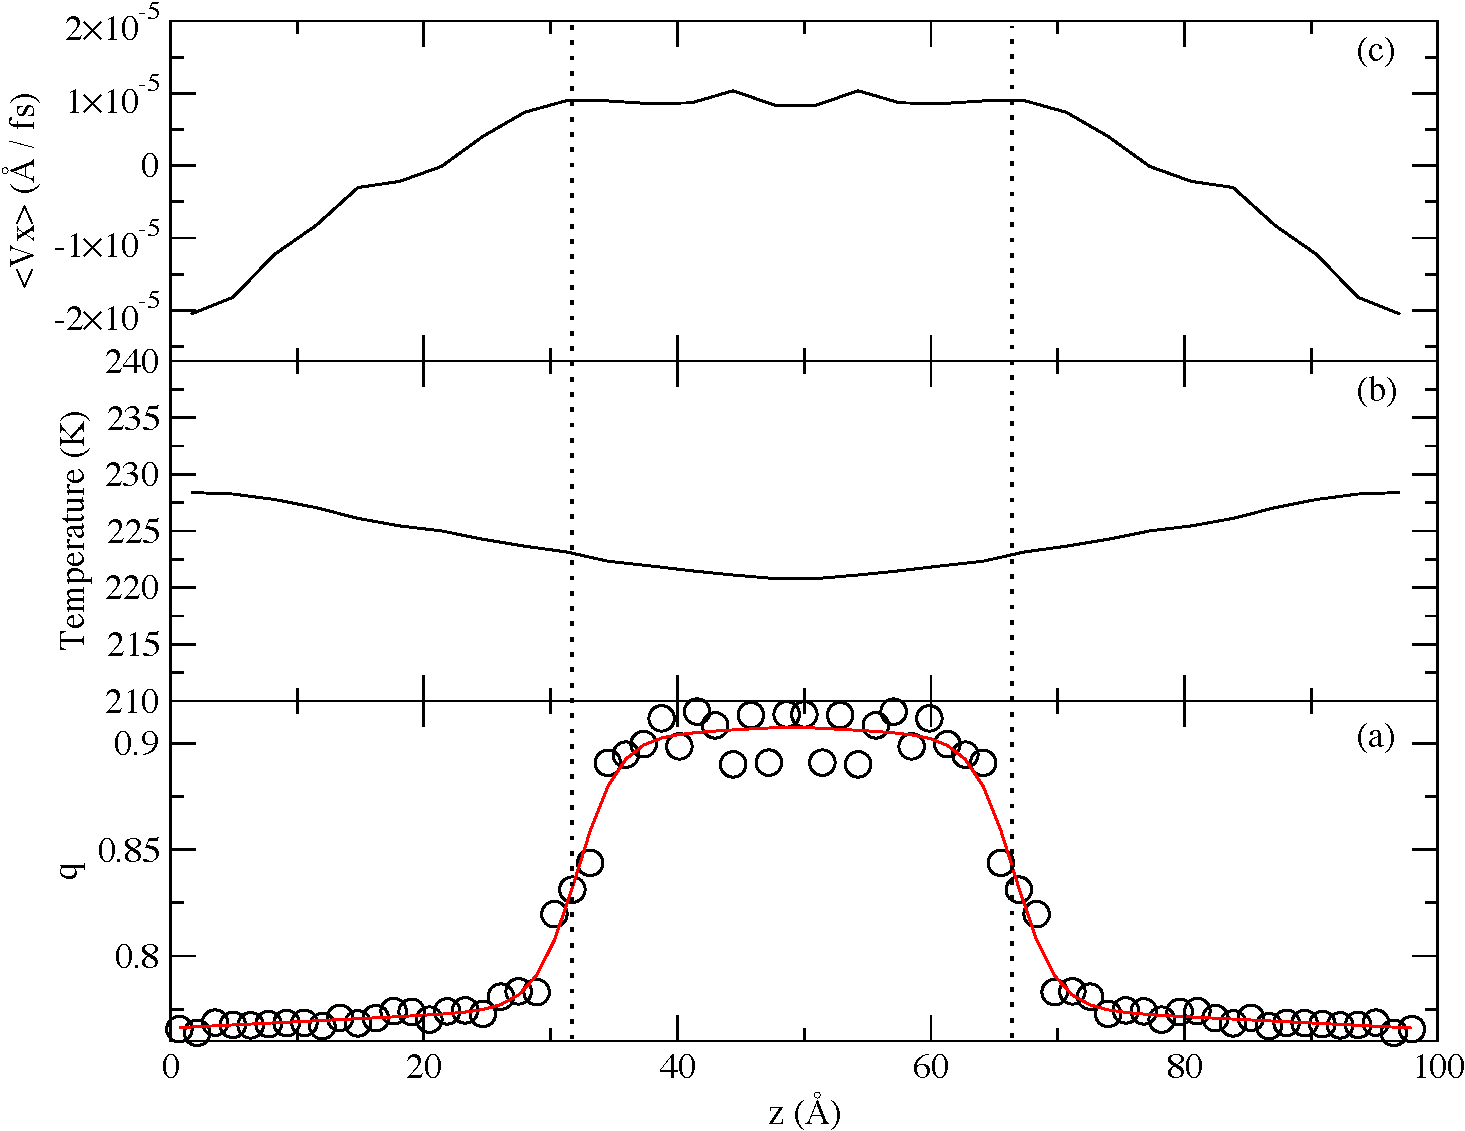
\includegraphics[width=\linewidth]{Figures/bComicStrip}
\caption{\label{fig:bComic} The basal interface with a shear rate of
  1.3 ms\textsuperscript{-1}.  Lower panel: the local tetrahedral order parameter, $q(z)$,
  (black circles) and the hyperbolic tangent fit (red line).  Middle
  panel: the imposed thermal gradient required to maintain a fixed
  interfacial temperature.  Upper panel: the transverse velocity
  gradient that develops in response to an imposed momentum flux.  The
  vertical dotted lines indicate the locations of the midpoints of the
  two interfaces.}
\end{figure}

\begin{figure}
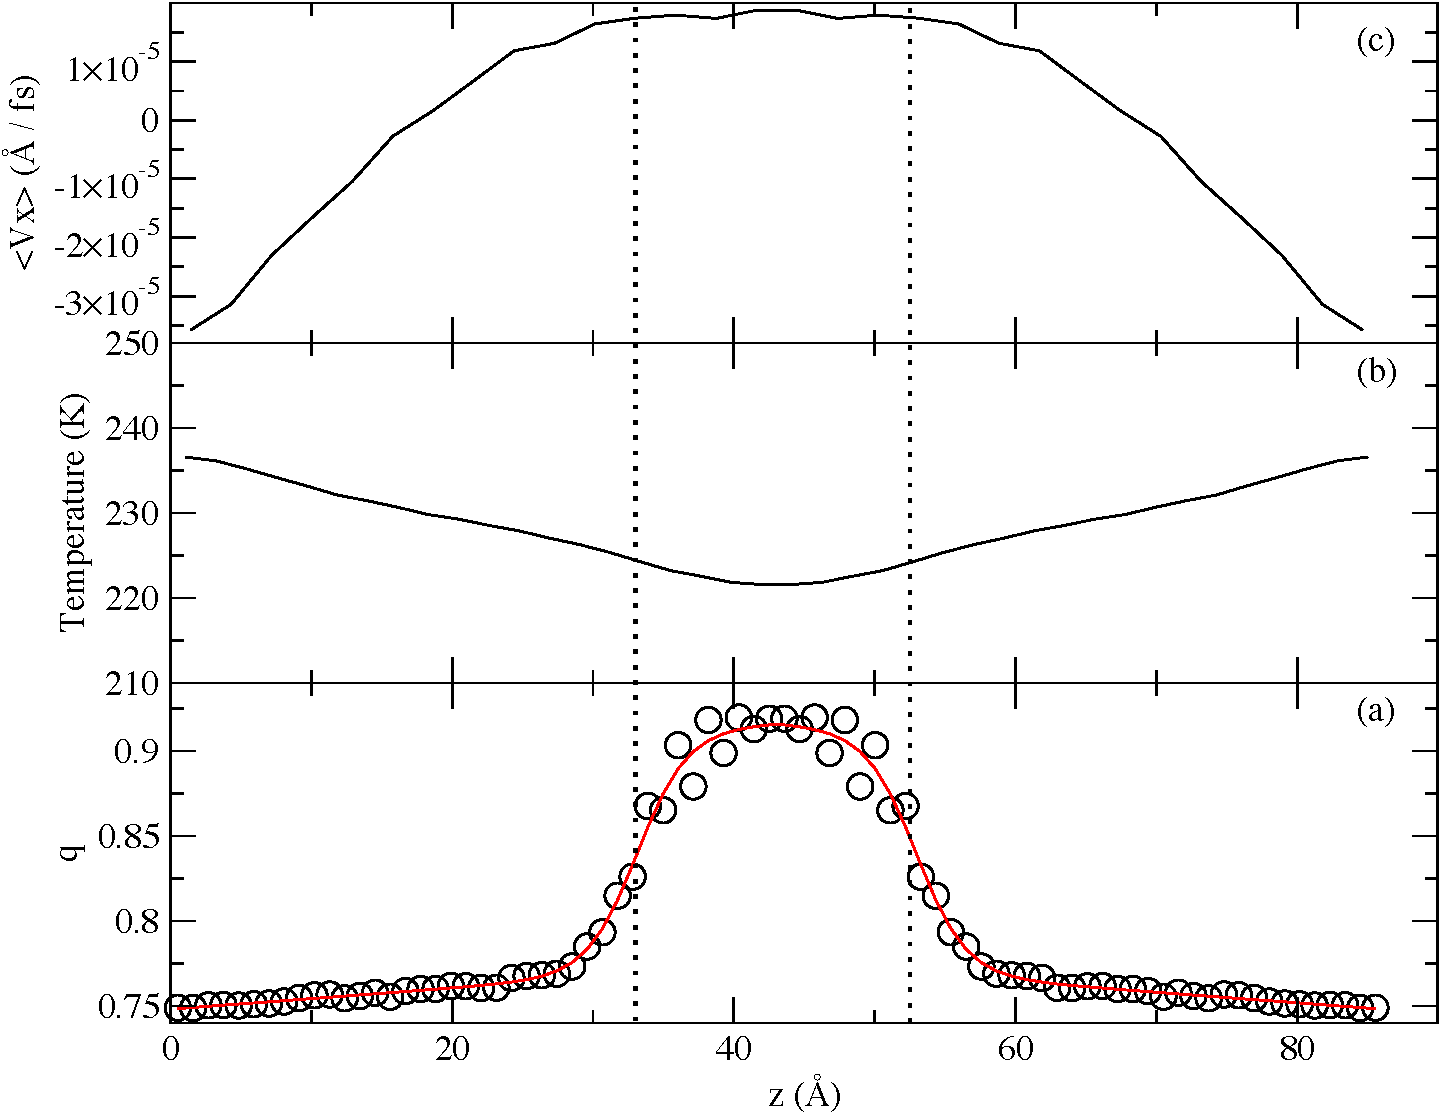
\includegraphics[width=\linewidth]{Figures/pComicStrip}
\caption{\label{fig:pComic} The prismatic interface with a shear rate
  of 2.0 ms\textsuperscript{-1}.  Panel
  descriptions match those in figure \ref{fig:bComic}}
\end{figure}

From the fits using eq. \eqref{tet_fit}, we find the interfacial width
for the basal and prismatic systems to be 3.2~$\pm$~0.4~\AA\ and
3.6~$\pm$~0.2~\AA\ , respectively, with no applied momentum flux. Over
the range of shear rates investigated, $0.6 \pm 0.3 \mathrm{ms}^{-1}
\rightarrow 5.3 \pm 0.5 \mathrm{ms}^{-1}$ for the basal system and
$0.9 \pm 0.2 \mathrm{ms}^{-1} \rightarrow 4.5 \pm 0.1
\mathrm{ms}^{-1}$ for the prismatic, we found no appreciable change in
the interface width. The fit values for the interfacial width ($w$)
over all shear rates contained the values reported above within their
error bars.  Note that the interfacial widths reported here are based
on the hyperbolic tangent parameter $w$ in Eq. \ref{tet_fit}.  This is
related to, but not identical with, the 10\%-90\% intefacial widths
commonly used in previous studies.\cite{Bryk02,Bryk2004b} To estimate
the 10\%-90\% widths, it is a simple matter to scale the widths
obtained from the hyperbolic tangent fits to obtain $w_{10-90} =
2.1971 \times w$.\cite{Bryk02,Bryk2004b} This results in $w_{10-90}$
values of 7.0~$\pm$~0.9~\AA\ for the basal face, and 7.9~$\pm$~0.4
\AA\ for the prismatic face.  These are somewhat smaller than
previously reported values.

\begin{figure}
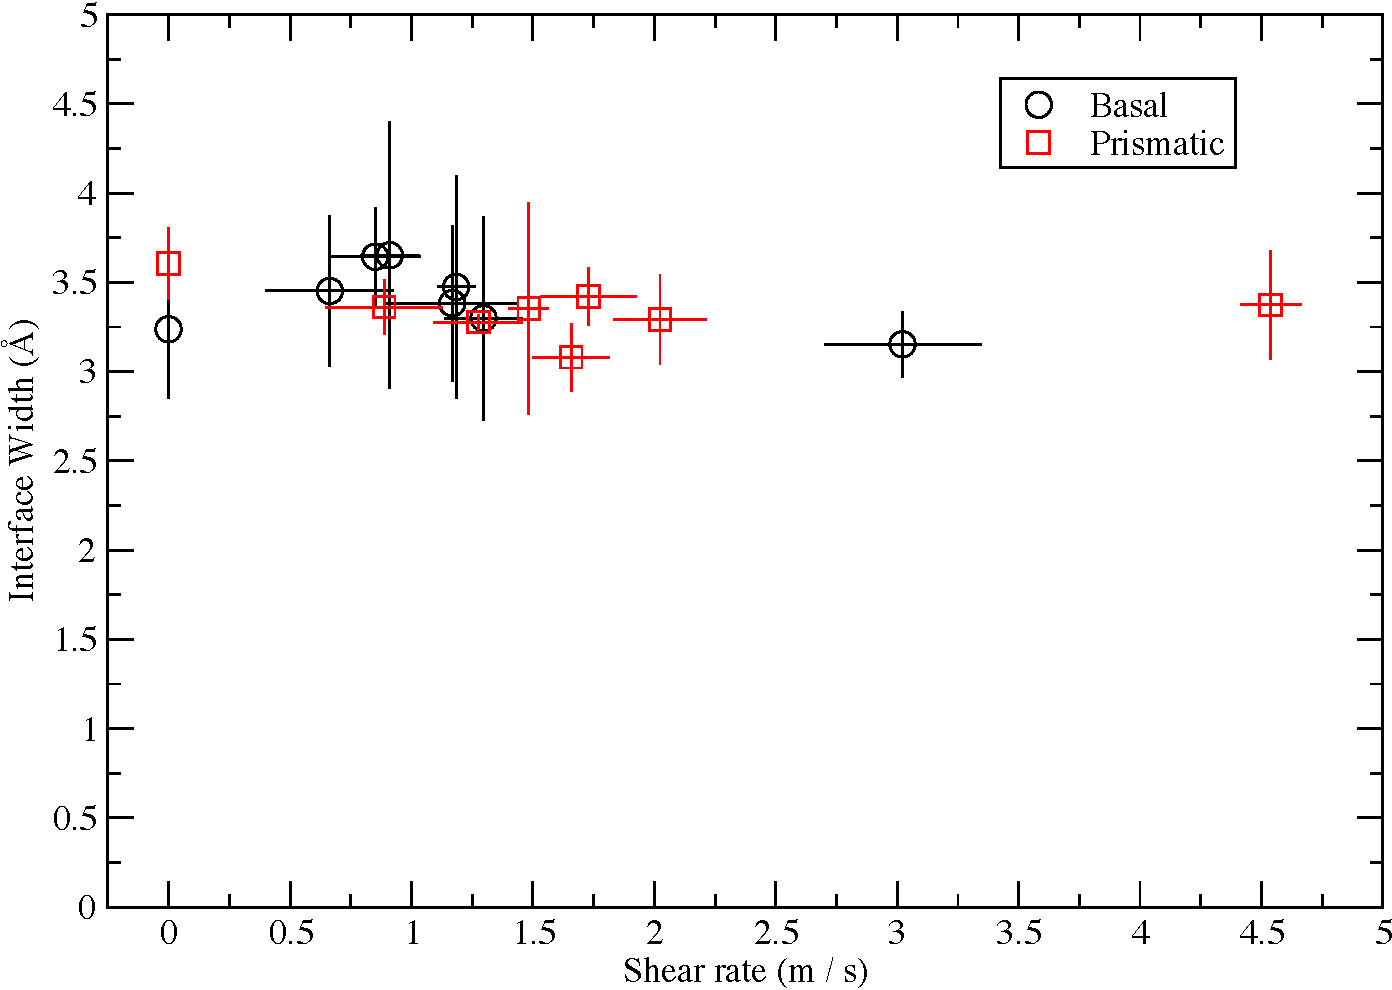
\includegraphics[width=\linewidth]{Figures/interface_width_by_shear_rate}
\caption{\label{fig:widthByShear} The width of the ice water
  interfaces (as measured by Eq. \ref{tet_fit}) exhibits no dependence
  on the applied shear rate between the ice and water regions.}
\end{figure}



\subsubsection{Orientational Dynamics}
The orientational time correlation function,
\begin{equation}\label{C(t)1}
  C_{2}(t)=\langle P_{2}(\mathbf{u}(0) \cdot \mathbf{u}(t)) \rangle,
\end{equation}
gives insight into the local dynamic environment around the water
molecules.  The rate at which the function decays provides information
about hindered motions and the timescales for relaxation.  In
eq. \eqref{C(t)1}, $P_{2}$ is the second-order Legendre polynomial,
the vector $\mathbf{u}$ is often taken as HOH bisector, although
slightly different behavior can be observed when $\mathbf{u}$ is the
vector along one of the OH bonds.  The angle brackets denote an
ensemble average over all water molecules in a given spatial region.

To investigate the dynamic behavior of water at the ice interfaces, we
have computed $C_{2}(z,t)$ for molecules that are present within a
particular slab along the $z$- axis at the initial time.  The change
in the decay behavior as a function of the $z$ coordinate is another
measure of the change of how the local environment changes across the
ice/water interface.  To compute these correlation functions, each of
the 0.5 ns simulations was followed by a shorter 200 ps microcanonical
(NVE) simulation in which the positions and orientations of every
molecule in the system were recorded every 0.1 ps. The systems were
then divided into 30 bins along the $z$-axis and $C_2(t)$ was
evaluated for each bin.

In simulations of water at biological interfaces, Furse {\em et al.}
fit $C_2(t)$ functions for water with triexponential
functions,\cite{Furse08} where the three components of the decay
correspond to a fast ($<$200 fs) reorientational piece driven by the
restoring forces of existing hydrogen bonds, a middle (on the order of
several ps) piece describing the large angle jumps that occur during
the breaking and formation of new hydrogen bonds,and a slow (on the
order of tens of ps) contribution describing the translational motion
of the molecules.  The model for orientational decay presented
recently by Laage and Hynes {\em et al.}\cite{Laage08,Laage11} also
includes three similar decay constants, although two of the time
constants are linked, and the resulting decay curve has two parameters
governing the dynamics of decay. 

In our ice/water interfaces, we are at substantially lower
temperatures, and the water molecules are further perturbed by the
presence of the ice phase nearby.  We have obtained the most
reasonable fits using triexponential functions with three distinct
time domains, as well as a constant piece to account for the water
stuck in the ice phase that does not experience any long-time
orientational decay,
\begin{equation}
C_{2}(t) \approx a e^{-t/\tau_\mathrm{short}} + b e^{-t/\tau_\mathrm{middle}} + c
e^{-t/\tau_\mathrm{long}} + (1-a-b-c)
\end{equation}
Average values for the three decay constants (and error estimates)
were obtained for each bin. In figures \ref{fig:basal_Tau_comic_strip}
and \ref{fig:prismatic_Tau_comic_strip}, the three orientational decay
times are shown as a function of distance from the center of the ice
slab.

\begin{figure}
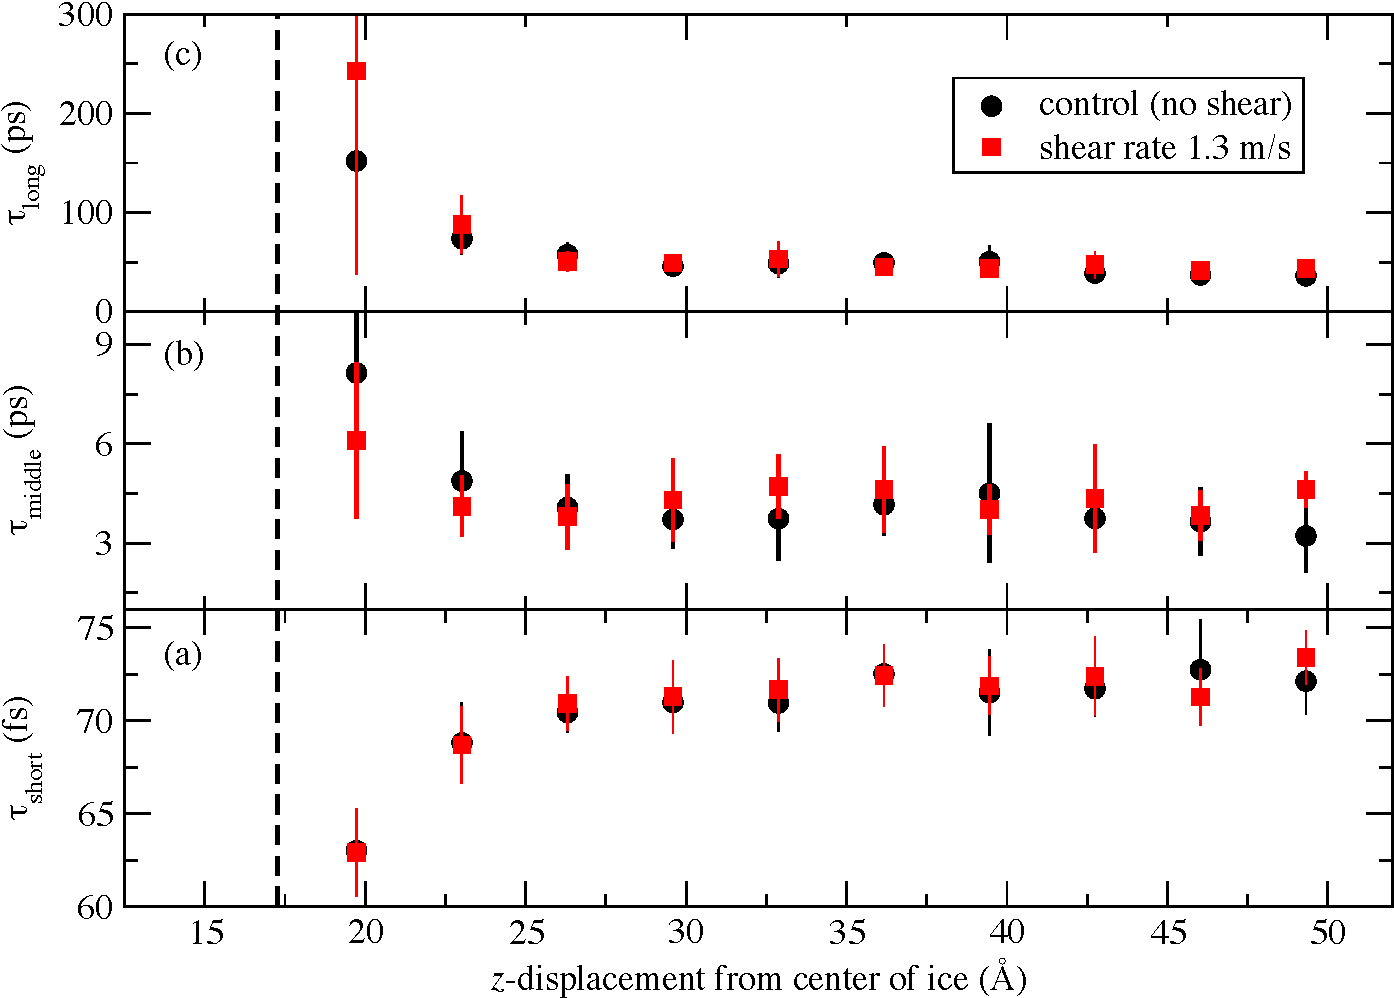
\includegraphics[width=\linewidth]{Figures/basal_Tau_comic_strip}
\caption{\label{fig:basal_Tau_comic_strip} The three decay constants
  of the orientational time correlation function, $C_2(t)$, for water
  as a function of distance from the center of the ice slab.  The
  dashed line indicates the location of the basal face (as determined
  from the tetrahedrality order parameter) and the black and red lines
  are fits of Eq. \ref{tauFit}.  The moderate and long
  time contributions slow down close to the interface which would be
  expected under reorganizations that involve large motions of the
  molecules (e.g. frame-reorientations and jumps).  The observed
  speed-up in the short time contribution is surprising, but appears
  to reflect the restricted motion of librations closer to the
  interface.}
\end{figure}

\begin{figure}
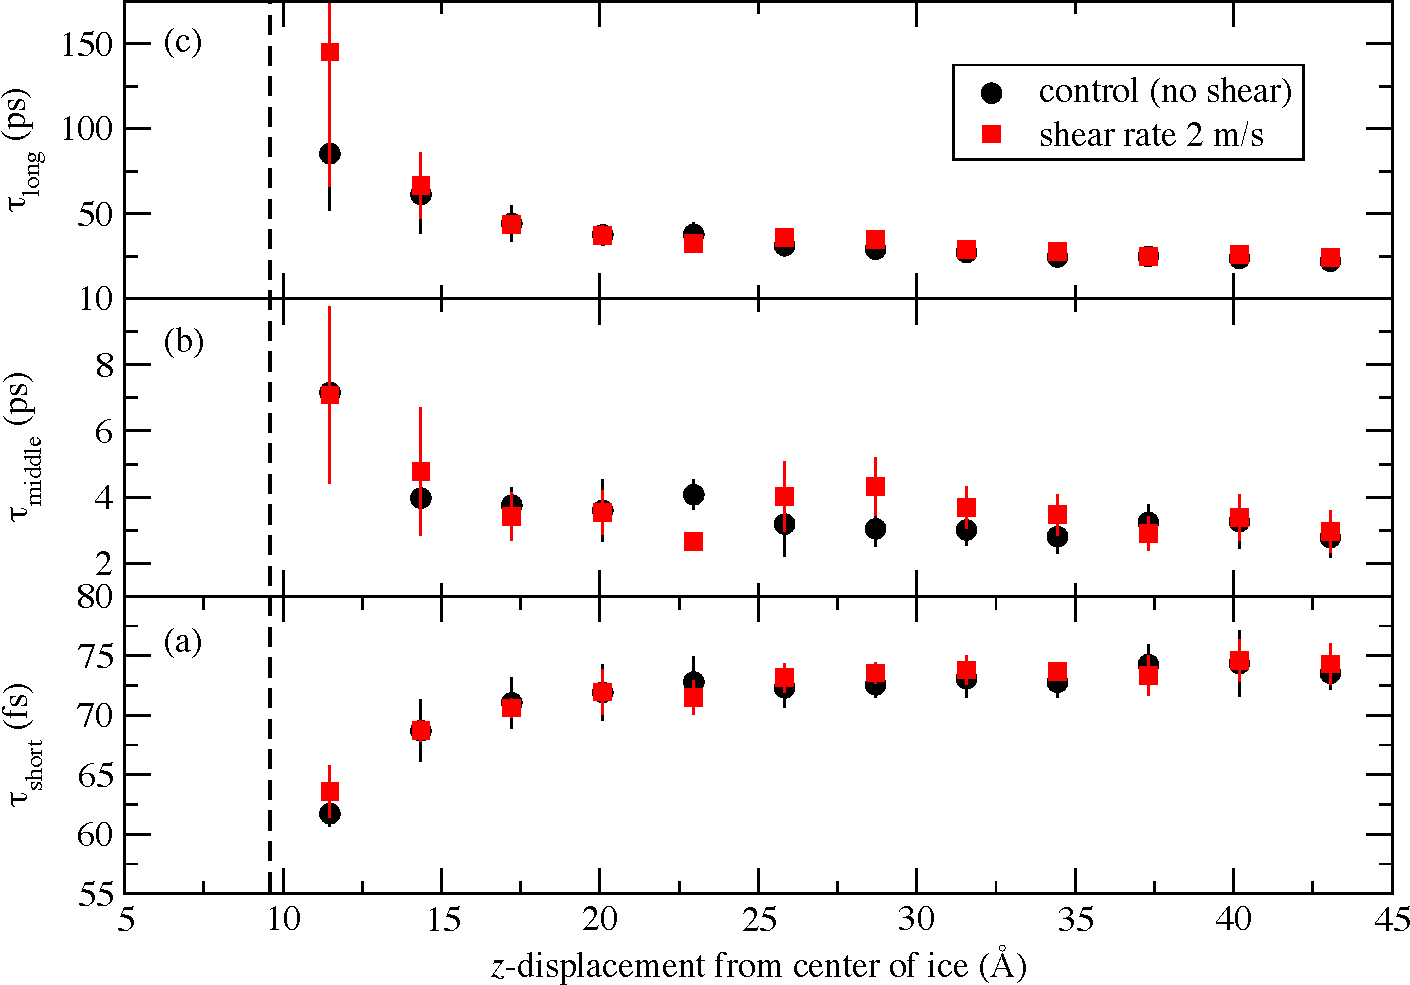
\includegraphics[width=\linewidth]{Figures/prismatic_Tau_comic_strip}
\caption{\label{fig:prismatic_Tau_comic_strip}
 Decay constants for $C_2(t)$ at the prismatic interface.  Panel
  descriptions match those in figure \ref{fig:basal_Tau_comic_strip}.}
\end{figure}

Figures \ref{fig:basal_Tau_comic_strip} and
\ref{fig:prismatic_Tau_comic_strip} show the three decay constants for
the orientational time correlation function for water at varying
displacements from the center of the ice slab for both the basal and
prismatic interfaces.  The vertical dotted lines indicate the
locations of the midpoints of the interfaces as determined by the
tetrahedrality fits. In the liquid regions, $\tau_{middle}$ and
$\tau_{long}$ have consistent values around 3-4 ps and 20-40 ps,
respectively, and increase in value approaching the interface.
According to the jump model of Laage and Hynes {\em et
  al.},\cite{Laage08,Laage11} $\tau_{middle}$ corresponds to the
breaking and making of hydrogen bonds and $\tau_{long}$ is explained
with translational motion of the molecules (i.e. frame reorientation).
The shortest of the three decay constants, the librational time
$\tau_\mathrm{short}$ has a value of about 70 fs in the liquid region,
and decreases in value approaching the interface. The observed
speed-up in the short time contribution is surprising, but appears to
reflect the restricted motion of librations closer to the interface.

The control systems (with no applied momentum flux) are shown with
black symbols in figs. \ref{fig:basal_Tau_comic_strip} and
\ref{fig:prismatic_Tau_comic_strip}, while those obtained while a
shear was active are shown in red.

Two notable features deserve clarification.  First, there are
nearly-constant liquid-state values for $\tau_{short}$,
$\tau_{middle}$, and $\tau_{long}$ at large displacements from the
interface. Second, there appears to be a single distance, $d_{basal}$
or $d_{prismatic}$, from the interface at which all three decay times
begin to deviate from their bulk liquid values. To quantify this
distance, each of the decay constant $z$-profiles were fit to
\begin{equation}\label{tauFit}
\tau(z)\approx\tau_{liquid}+(\tau_{solid}-\tau_{liquid})e^{-(z-z_{wall})/d}
\end{equation}
where $\tau_{liquid}$ and $\tau_{solid}$ are the liquid and projected
solid values of the decay constants, $z_{wall}$ is the location of the
interface, and $d$ is the displacement the deviations occur at (see
Figures \ref{fig:basal_Tau_comic_strip} and
\ref{fig:prismatic_Tau_comic_strip}). The displacements $d_{basal}$
and $d_{prismatic}$ were determined for each of the three decay
constants, and then averaged for better statistics.
For the basal system, we found $d_{basal}$ for the control set to be
2.9 \AA\, and 2.8 \AA\ for a simulation with a shear rate of 1.3
ms\textsuperscript{-1}. We found $d_{prismatic}$ to be slightly
larger than $d_{basal}$ for both the control and an applied shear,
with displacements of 3.6 \AA\ for the control system and 3.5 \AA\ for
a simulation with a 2 ms\textsuperscript{-1} shear rate. From this we
can conclude there is no apparent dependence on the shear rate for the dynamic interface
width. 

%%%%%%%%Should we keep this paragraph???%%%%%%%%%%%%%%%
Beaglehole and Wilson have measured the ice/water interface using
ellipsometry and find a thickness of approximately 10~\AA\ for both
the basal and prismatic faces.\cite{Beaglehole93} Structurally, we
have found the basal and prismatic interfacial width to be
3.2~$\pm$~0.4~\AA\ and 3.6~$\pm$~0.2~\AA.  Decomposition of
the spatial dependence of the decay times of $C_2(t)$ shows good
agreement with the structural interfacial width determined by the
local tetrahedrality.
%%%%%%%%%%%%%%%%%%%%%%%%%%%%%%%%%%%%%%%%%%%%%%


\subsection{Coefficient of Friction of the Interface}
As liquid water flows over an ice interface, there is a distance from
the structural interface where bulk-like hydrodynamics are recovered.
Bocquet and Barrat constructed a theory for the hydrodynamic boundary
parameters, which include the slipping length
$\left(\delta_\mathrm{wall}\right)$ of this boundary layer and the
``hydrodynamic position'' of the boundary
$\left(z_\mathrm{wall}\right)$.\cite{PhysRevLett.70.2726,PhysRevE.49.3079}
This last parameter is the location (relative to a solid surface)
where the bulk-like behavior is recovered.  Work by Mundy {\it et al.}
has helped to combine these parameters into a liquid-solid friction
coefficient, which quantifies the resistance to pulling the solid
interface through a liquid,\cite{Mundy1997305}
\begin{equation}
\lambda_\mathrm{wall} = \frac{\eta}{\delta_\mathrm{wall}}.
\end{equation}
This expression is nearly identical to one provided by Pit {\it et
  al.} for the solid-liquid friction of an interface,\cite{Pit99}
\begin{equation}\label{Pit}
  \lambda=\frac{\eta}{\delta}
\end{equation}
where $\delta$ is the slip length for the liquid measured at the
location of the interface itself.  In our simulations, the shoulder on
the velocity profile indicating the location of the hydrodynamic
boundary in the liquid is not always apparent. In some cases, the
linear behavior persists nearly up to the interfacial region.  For
this reason, the hydrodynamic position of the boundary is not always
computable, while the Pit approach (Eq. \ref{Pit}) can be used to find
the solid-liquid friction coefficient more reliably.

In both the Pit and hydrodynamic boundary expressions, $\eta$ is the
shear viscosity of the bulk-like region of the liquid, a quantity
which is easily obtained in VSS-RNEMD simulations by fitting the
velocity profile in the region far from the surface.\cite{Kuang12}
Assuming linear response in the bulk-like region,
\begin{equation}\label{Kuang}
j_{z}(p_{x})=-\eta \left(\frac{\partial v_{x}}{\partial z}\right)
\end{equation}
Substituting this result into eq. \eqref{Pit}, we can estimate the
solid-liquid coefficient using the slip length,
\begin{equation}
\lambda=-\frac{j_{z}(p_{x})} {\left(\frac{\partial v_{x}}{\partial
      z}\right) \delta}
\end{equation}

For ice / water interfaces, the boundary conditions are no-slip, so
projecting the bulk liquid state velocity profile yields a negative
slip length. This length is the difference between the structural edge
of the ice (determined by the tetrahedrality profile) and the location
where the projected velocity of the bulk liquid intersects the solid
phase velocity (see Figure \ref{fig:delta_example}). The coefficients
of friction for the basal and the prismatic facets were determined for
shearing along both the $x$ and $y$ axes.  The values are given in
table \ref{tab:lambda}. 

Note that the measured friction coefficient for the basal face is
twice that of the prismatic face (regardless of drag direction).
These results may seem surprising as the basalface appears smoother
than the prismatic with only small undulations of the oxygen
positions, while the prismatic surface has deep corrugated channels
along the $x$ direction in the crystal system used in this work.
However, the corrugations are relatively thin, and the liquid phase
water does not appear to populate the channels.  The prismatic face
therefore effectively presents stripes of solid-phase molecules
(making up approximately half of the exposed surface area) with nearly
empty space between them. The interfacial friction appears to be
independent of the drag direction, so flow parallel to these channels
does not explain the lower friction of the prismatic face.  A more
likely explanation is that the effective contact between the liquid
phase and the prismatic face is reduced by the empty corrugations.  

\begin{figure}
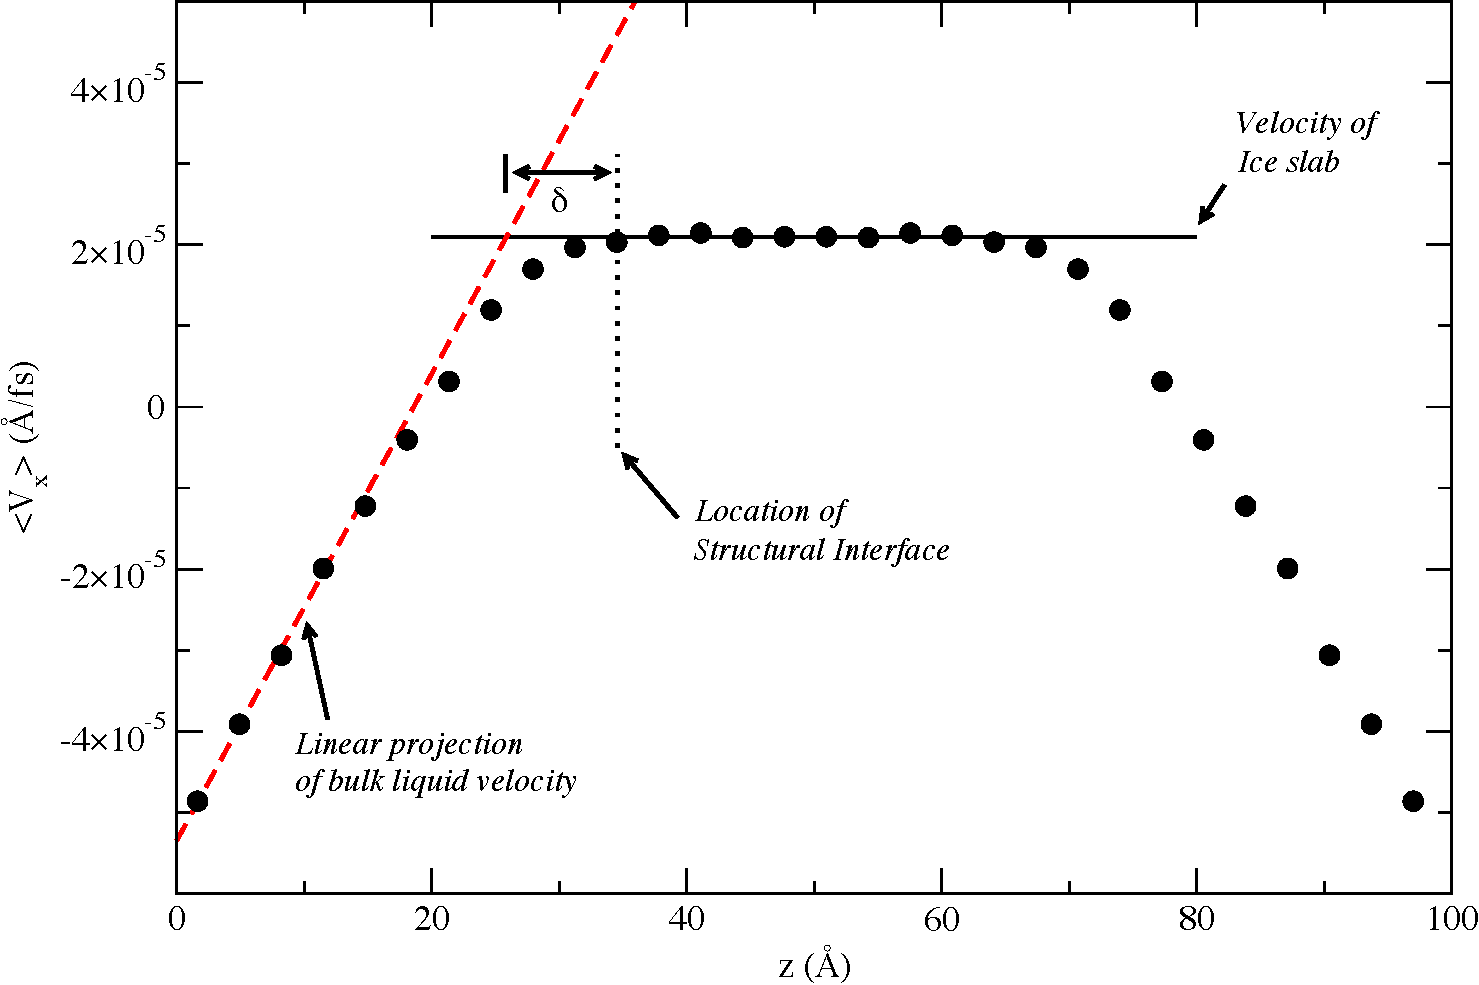
\includegraphics[width=\linewidth]{Figures/delta_example}
\caption{\label{fig:delta_example} Determining the (negative) slip
  length ($\delta$) for the ice-water interfaces (which have decidedly
  non-slip behavior).  This length is the difference between the
  structural edge of the ice (determined by the tetrahedrality
  profile) and the location where the projected velocity of the bulk
  liquid (dashed red line) intersects the solid phase velocity (solid
  black line).  The dotted line indicates the location of the ice as
  determined by the tetrahedrality profile.  This example is taken
  from the basal-face simulation with an applied shear rate of 3.0 ms\textsuperscript{-1}.}
\end{figure}


\begin{table}[h]
\centering
\caption{Solid-liquid friction coefficients (measured in amu~fs\textsuperscript{-1}) }
\label{tab:lambda}
\begin{tabular}{|ccc|}  \hline
           & \multicolumn{2}{c|}{Drag direction} \\ 
 Interface & $x$               & $y$  \\ \hline
     basal &  $0.08 \pm 0.02$  & $0.09 \pm 0.03$ \\
 prismatic & $0.037 \pm 0.008$ & $0.04 \pm 0.01$ \\ \hline
\end{tabular}
\end{table}


\section{Conclusion}
We have simulated the basal and prismatic facets of an SPC/E model of
the ice I$_\mathrm{h}$ / water interface.  Using VSS-RNEMD, the ice
was sheared relative to the liquid while simultaneously being exposed
to a weak thermal gradient which kept the interface at a stable
temperature.  Calculation of the local tetrahedrality order parameter
has shown an apparent independence of the interfacial width on the
shear rate.  This width was found to be 3.2~$\pm$0.4~\AA\ and
3.6~$\pm$0.2~\AA\ for the basal and prismatic systems, respectively.

Orientational time correlation functions were calculated at varying
displacements from the interface, and were found to be similarly
independent of the applied momentum flux. The short decay due to the
restoring forces of existing hydrogen bonds decreased close to the
interface, while the longer-time decay constants increased in close
proximity to the interface.  There is also an apparent dynamic
interface width, $d_{basal}$ and $d_{prismatic}$, at which these
deviations from bulk liquid values begin.  We found $d_{basal}$ and
$d_{prismatic}$ to be approximately 2.8~\AA\ and 3.5~\AA\ . This
interfacial width is in good agreement with values determined by the
structural analysis of the interface, by the hyperbolic tangent fit of
the local tetrahedral order parameter.

The coefficient of liquid-solid friction for each of the facets was
also determined. They were found to be
0.07~$\pm$~0.01~amu~fs\textsuperscript{-1} and
0.032~$\pm$~0.007~amu~fs\textsuperscript{-1} for the basal and
prismatic facets respectively. We attribute the large difference
between the two friction coefficients to the direction of the shear
and to the surface structure of the crystal facets.



\message{ !name(iceWater.tex) !offset(-705) }
